% ============================================================================
% Appendix E: Topological Entanglement Entropy --- Derivation
% ============================================================================
%
% Purpose
%   Derive the universal subleading correction gamma = log D to the
%   entanglement entropy of a topologically ordered ground state, using
%   the Kitaev-Preskill subtraction scheme.
%
% References
%   Kitaev-Preskill 2006 (\cite{KitaevPreskill2006TEE})
%   Levin-Wen 2006 (\cite{LevinWen2006DetectingTO})

\section{Topological Entanglement Entropy: Derivation}
\label{app:tee}

This appendix derives the topological entanglement entropy formula stated in Section~\ref{subsec:lre-vs-symmetry-breaking}, following the approach of Kitaev and Preskill \cite{KitaevPreskill2006TEE} (see also Levin and Wen \cite{LevinWen2006DetectingTO} for an equivalent construction with a different region geometry).

\medskip
\noindent\textbf{Setup and assumptions.}
Consider a topologically ordered ground state $\ket{\Psi}$ on a two-dimensional lattice, and let $A$ be a simply-connected disk-like region whose boundary $\del A$ is smooth on the scale of the correlation length $\xi$.  We assume:
\begin{enumerate}
    \item The system is gapped with correlation length $\xi$.
    \item The region $A$ is large compared to $\xi$, so that the boundary length satisfies $|\del A| \gg \xi$.
    \item The ground state has no long-range correlations beyond the topological sector (i.e., connected correlation functions of local operators decay exponentially with characteristic length $\xi$).
\end{enumerate}

Under these conditions, the von Neumann entanglement entropy $S(A) = -\Tr(\rho_A \log \rho_A)$, with $\rho_A = \Tr_{\bar{A}} \ket{\Psi}\!\bra{\Psi}$, admits an expansion
\begin{equation}\label{eq:tee-expansion}
    S(A) \;=\; \alpha\, |\del A| \;-\; \gamma \;+\; O(|\del A|^{-1}),
\end{equation}
where $\alpha$ is a non-universal coefficient depending on microscopic details near the boundary.  Our goal is to extract the universal constant $\gamma$ by a subtraction that eliminates $\alpha$.

\medskip
\noindent\textbf{The Kitaev--Preskill subtraction scheme.}
The difficulty in extracting $\gamma$ directly from \eqref{eq:tee-expansion} is that $\alpha$ is unknown and region-dependent.  Kitaev and Preskill resolve this by considering a partition of the disk $A$ into three sectors $A_1$, $A_2$, $A_3$ meeting at a single point in the interior, so that the full disk is $A = A_1 \cup A_2 \cup A_3$ (see Figure~\ref{fig:kp-geometry}).  Define the combination
\begin{equation}\label{eq:kp-combination}
    S_{\mathrm{topo}} \;=\; S(A_1) + S(A_2) + S(A_3) - S(A_1 A_2) - S(A_2 A_3) - S(A_1 A_3) + S(A_1 A_2 A_3),
\end{equation}
where $S(X)$ denotes the entanglement entropy of region $X$ and $A_i A_j$ denotes the union $A_i \cup A_j$.

The key observation is that the area-law contribution $\alpha |\del X|$ is \emph{extensive} in the boundary length.  Each segment of boundary between two regions is shared: it appears with a positive sign in some terms and a negative sign in others.  By the inclusion-exclusion structure of \eqref{eq:kp-combination}, every boundary segment---both the internal boundaries between sectors and the external boundary of the disk---cancels exactly.  Schematically, if $\ell_{ij}$ denotes the length of the boundary between $A_i$ and $A_j$, and $\ell_i^{\mathrm{ext}}$ the external boundary of $A_i$, then the area-law contributions satisfy
\begin{equation}\label{eq:boundary-cancellation}
    \alpha\bigl[(\ell_1^{\mathrm{ext}} + \ell_{12} + \ell_{13}) + (\ell_2^{\mathrm{ext}} + \ell_{12} + \ell_{23}) + (\ell_3^{\mathrm{ext}} + \ell_{13} + \ell_{23}) - \cdots \bigr] = 0,
\end{equation}
where the cancellation holds term by term for each boundary segment.

What survives is the topological contribution.  For a simply-connected region $X$ in a topologically ordered phase, the subleading correction is $-\gamma$, while for a region with a more complex topology the correction depends on how many disconnected boundary components it has.  Since each $A_i$ is simply connected and each pairwise union $A_i A_j$ is also simply connected (the sectors share boundaries), but the full disk $A_1 A_2 A_3$ is also simply connected, the topological terms contribute
\begin{equation}\label{eq:topo-extraction}
    S_{\mathrm{topo}} \;=\; 3(-\gamma) - 3(-\gamma) + (-\gamma) \;=\; -\gamma.
\end{equation}

\begin{figure}[ht]
\centering
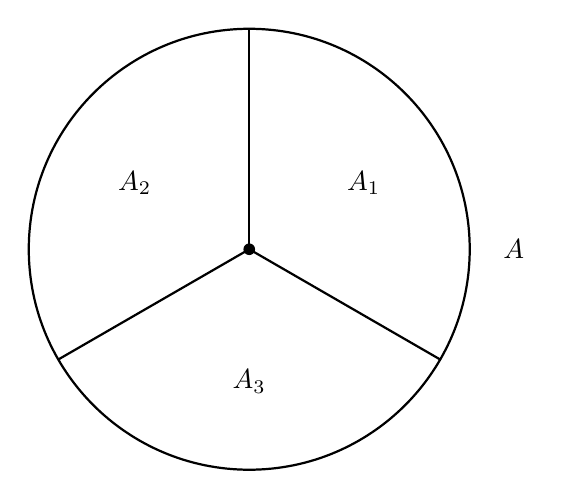
\begin{tikzpicture}[scale=1.4]
    % Disk boundary
    \draw[thick] (0,0) circle (2cm);
    % Internal boundaries (radial lines from center to boundary)
    \draw[thick] (0,0) -- (90:2);
    \draw[thick] (0,0) -- (210:2);
    \draw[thick] (0,0) -- (330:2);
    % Region labels
    \node at (30:1.2) {$A_1$};
    \node at (150:1.2) {$A_2$};
    \node at (270:1.2) {$A_3$};
    % Center point
    \fill (0,0) circle (1.5pt);
    % External boundary label
    \node at (0:2.4) {$\del A$};
\end{tikzpicture}
\caption{The Kitaev--Preskill disk partition.  The simply-connected region $A$ is divided into three sectors $A_1, A_2, A_3$ meeting at a single interior point.  The subtraction scheme \eqref{eq:kp-combination} cancels all boundary-length-dependent terms, isolating the topological correction $-\gamma$.}
\label{fig:kp-geometry}
\end{figure}

\begin{remark}\label{rmk:levin-wen}
Levin and Wen \cite{LevinWen2006DetectingTO} use an annular geometry instead, dividing a ring into four regions and constructing a similar linear combination.  The two schemes give identical results for the universal piece; they differ only in the shape of subleading finite-size corrections.
\end{remark}

\medskip
\noindent\textbf{Relating $\gamma$ to the total quantum dimension.}
To identify $\gamma$ with the total quantum dimension $\mathcal{D}$, we use the structure of the reduced density matrix in a topologically ordered phase.  The key input is that, for a disk-like region $A$ in a state belonging to a definite anyon sector $a$ threading the boundary, the entanglement entropy receives a contribution from the anyonic superselection structure.  Specifically, the reduced density matrix decomposes into superselection sectors labeled by the anyon type $a$ that crosses $\del A$:
\begin{equation}\label{eq:superselection-decomp}
    \rho_A \;=\; \bigoplus_a p_a \,\rho_A^{(a)},
\end{equation}
where $p_a = d_a^2 / \mathcal{D}^2$ is the probability of finding sector $a$ at the boundary, with $d_a$ the quantum dimension of anyon $a$.

The von Neumann entropy then splits into two parts: the Shannon entropy of the sector probabilities and a weighted sum of within-sector entropies:
\begin{equation}\label{eq:entropy-split}
    S(A) \;=\; -\sum_a p_a \log p_a \;+\; \sum_a p_a \, S(\rho_A^{(a)}) \;+\; \alpha\,|\del A|.
\end{equation}
The within-sector entropies and the last term contribute only area-law pieces.  The Shannon term gives
\begin{equation}\label{eq:shannon-piece}
    -\sum_a p_a \log p_a \;=\; -\sum_a \frac{d_a^2}{\mathcal{D}^2} \log \frac{d_a^2}{\mathcal{D}^2} \;=\; \log \mathcal{D}^2 - \frac{2}{\mathcal{D}^2}\sum_a d_a^2 \log d_a.
\end{equation}
For the ground state on a disk (vacuum sector threading the boundary), only the identity sector $a = 1$ with $d_1 = 1$ contributes at leading order, and a more careful analysis using the entanglement structure of the topological vacuum shows that the universal correction is
\begin{equation}\label{eq:gamma-result}
    \gamma \;=\; \log \mathcal{D}, \qquad \mathcal{D} \;=\; \sqrt{\sum_a d_a^2}.
\end{equation}

\medskip
\noindent\textbf{Verification: toric code.}
For the $\Z_2$ toric code, the anyon content is $\{1, e, m, \epsilon\}$ with quantum dimensions $d_a = 1$ for all four sectors (cf.\ Section~\ref{subsec:emergent-anyons}).  Thus
\begin{equation}\label{eq:tee-toric-check}
    \mathcal{D} = \sqrt{1 + 1 + 1 + 1} = 2, \qquad \gamma = \log 2.
\end{equation}
This matches the direct lattice calculation of the entanglement entropy of the toric code ground state, confirming the general formula.

\medskip
\noindent\textbf{Example: Laughlin states at $\nu = 1/m$.}
The Laughlin state at filling fraction $\nu = 1/m$ (with $m$ odd) is described by a $U(1)_m$ Chern--Simons theory.  The anyon content consists of $m$ sectors $\{a_0, a_1, \ldots, a_{m-1}\}$, each with quantum dimension $d_{a_k} = 1$ (all anyons are abelian).  The total quantum dimension is therefore
\begin{equation}\label{eq:tee-laughlin}
    \mathcal{D} = \sqrt{\sum_{k=0}^{m-1} 1^2} = \sqrt{m}, \qquad \gamma = \tfrac{1}{2}\log m.
\end{equation}
For the $\nu = 1/3$ state relevant to the fractional quantum Hall effect, this gives $\gamma = \frac{1}{2}\log 3$, while the integer quantum Hall state $m = 1$ has $\mathcal{D} = 1$ and $\gamma = 0$---correctly reflecting the absence of topological order (the state has a single sector and no long-range entanglement).

\medskip
\noindent\textbf{Example: Ising topological order.}
The Ising anyon model has three sectors $\{1, \sigma, \psi\}$ with quantum dimensions $d_1 = 1$, $d_\sigma = \sqrt{2}$, and $d_\psi = 1$.  The total quantum dimension is
\begin{equation}\label{eq:tee-ising}
    \mathcal{D} = \sqrt{d_1^2 + d_\sigma^2 + d_\psi^2} = \sqrt{1 + 2 + 1} = 2, \qquad \gamma = \log 2.
\end{equation}
Notably, $\mathcal{D} = 2$ coincides with the toric code value, despite the two theories having different anyon content (in particular, $\sigma$ is non-abelian with $d_\sigma = \sqrt{2}$, while all toric code anyons are abelian).  This illustrates that $\gamma$ alone does not uniquely identify the topological order---it is a necessary but not sufficient diagnostic.  Distinguishing the Ising model from the toric code requires additional invariants such as the modular $S$-matrix or the chiral central charge.

\medskip
\noindent\textbf{Physical interpretation.}
The topological entanglement entropy $\gamma = \log \mathcal{D}$ quantifies the ``missing information'' in the reduced density matrix due to long-range entanglement.  A local observer with access only to region $A$ cannot determine which topological sector the full state occupies; this ignorance manifests as a \emph{reduction} in entropy relative to the naive area law (note the minus sign in \eqref{eq:tee-expansion}).  The greater the total quantum dimension---i.e., the richer the anyon content---the larger this universal deficit.  Since $\gamma$ depends only on the quantum dimensions $\{d_a\}$, it is a topological invariant of the phase: it cannot change without a phase transition that closes the gap.
